\documentclass[10pt]{article}

% Packages and macros go here
\usepackage[T1]{fontenc}
\usepackage{lmodern}
\usepackage[utf8]{inputenc}
\usepackage{microtype}
\usepackage{framed}
\usepackage{listings}
\usepackage{vmargin}
\usepackage{setspace}
\usepackage{mathrsfs, mathenv}
\usepackage{amsmath, amsthm, amssymb, amsfonts, amscd}
\usepackage{graphicx}
\usepackage{epstopdf}
\usepackage[svgnames]{xcolor}
\usepackage{hyperref}
\hypersetup{citecolor=blue, colorlinks=true, linkcolor=black}
%\usepackage[capitalise]{cleveref}
\setlength{\parskip}{6pt}
\setlength\parindent{0pt}
\usepackage{subcaption}
\usepackage{bbm}
\usepackage{cite}
\usepackage{verbatim}
\usepackage{pgfplots}
\usepackage{tikz}
\usetikzlibrary{arrows,decorations.pathmorphing,backgrounds,positioning,fit,matrix}
\usepackage{etoolbox}
\usepackage{color}
\usepackage{lipsum}
\usepackage{ifthen}
\usepackage[ruled, vlined]{algorithm2e}
\usepackage[title]{appendix}

%\usepackage[capitalise]{cleveref}
%\crefname{algocf}{Algorithm}{Algorithms}

\theoremstyle{plain}
\newtheorem{theorem}{Theorem}[section]
\newtheorem{corollary}[theorem]{Corollary}
\newtheorem{lemma}[theorem]{Lemma}
\newtheorem{proposition}[theorem]{Proposition}
\numberwithin{equation}{section}

\theoremstyle{definition}
\newtheorem{definition}{Definition}

\theoremstyle{remark}
\newtheorem{remark}[theorem]{Remark}
\newtheorem{assumption}[theorem]{Assumption}
\newtheorem{example}[theorem]{Example}


\ifpdf
  \DeclareGraphicsExtensions{.eps,.pdf,.png,.jpg}
\else
  \DeclareGraphicsExtensions{.eps}
\fi

\usepackage{mathtools}
\mathtoolsset{showonlyrefs}

% basics

% tables
\usepackage{booktabs}

% plots
\usepackage{pgfplots}
\usepackage{tikz}
\usetikzlibrary{patterns,arrows,decorations.pathmorphing,backgrounds,positioning,fit,matrix}
\usepackage[labelfont=bf]{caption}
\setlength{\belowcaptionskip}{-5pt}
\usepackage{here}
\usepackage[font=normal]{subcaption}

% Prevent itemized lists from running into the left margin inside theorems and proofs
\usepackage{enumitem}
\setlist[itemize]{leftmargin=.5in}
\setlist[enumerate]{leftmargin=.5in,topsep=3pt,itemsep=3pt,label=(\roman*)}

% Add a serial/Oxford comma by default.
\newcommand{\creflastconjunction}{, and~}

% Sets running headers as well as PDF title and authors
% title and authors
\newcommand*\samethanks[1][\value{footnote}]{\footnotemark[#1]}

\newcommand{\email}[1]{\href{#1}{#1}}
\newcommand{\TheTitle}{Model Misspecification and Uncertainty Quantification \\ for Drift Estimation in Multiscale Diffusion Processes} 
\newcommand{\TheAuthors}{A. Abdulle, G. Garegnani, G. Pavliotis, A. M. Stuart}
\title{\TheTitle}
\author{Assyr Abdulle \thanks{Institute of Mathematics, École Polytechnique Fédérale de Lausanne}
		\and Giacomo Garegnani  \samethanks
		\and Grigorios A. Pavliotis \thanks{Department of Mathematics, Imperial College London}
		\and Andrew M. Stuart \thanks{Department of Computing and Mathematical Sciences, Caltech}
		\and Andrea Zanoni \samethanks[1]
}
\date{}
%\title{Caltech notes}
%\author{Giacomo Garegnani}
%\date{}

\usepackage{amsopn}
\DeclareMathOperator{\diag}{diag}
\DeclarePairedDelimiter{\ceil}{\left\lceil}{\right\rceil}
\DeclarePairedDelimiter{\floor}{\lfloor}{\rfloor}
\newcommand{\abs}[1]{\left\lvert#1\right\rvert}
\newcommand{\norm}[1]{\left\|#1\right\|}
\renewcommand{\phi}{\varphi}
\renewcommand{\theta}{\vartheta}
\renewcommand{\Pr}{\mathbb{P}}
\newcommand{\btilde}{\widetilde}
\newcommand{\bhat}{\widehat}
\newcommand{\eqtext}[1]{\ensuremath{\stackrel{#1}{=}}}
\newcommand{\leqtext}[1]{\ensuremath{\stackrel{#1}{\leq}}}
\newcommand{\iid}{\ensuremath{\stackrel{\text{i.i.d.}}{\sim}}}
\newcommand{\totext}[1]{\ensuremath{\stackrel{#1}{\to}}}
\newcommand{\rightarrowtext}[1]{\ensuremath{\stackrel{#1}{\longrightarrow}}}
\newcommand{\leftrightarrowtext}[1]{\ensuremath{\stackrel{#1}{\longleftrightarrow}}}
\newcommand{\pdv}[2]{\ensuremath\partial_{#2}#1}
\newcommand{\N}{\mathbb{N}}
\newcommand{\R}{\mathbb{R}}
\newcommand{\C}{\mathbb{C}}
\newcommand{\OO}{\mathcal{O}}
\newcommand{\epl}{\varepsilon}
\newcommand{\diffL}{\mathcal{L}}
\newcommand{\defeq}{\coloneqq}
\newcommand{\eqdef}{\eqqcolon}
\newcommand{\Var}{\operatorname{Var}}
\newcommand{\E}{\operatorname{\mathbb{E}}}
\newcommand{\PP}{\operatorname{\mathbb{P}}}
\newcommand{\MSE}{\operatorname{MSE}}
\newcommand{\trace}{\operatorname{tr}}
\newcommand{\MH}{\mathrm{MH}}
\newcommand{\ttt}{\texttt}
\newcommand{\Hell}{d_{\mathrm{Hell}}}
\newcommand{\sksum}{{\textstyle\sum}}
\renewcommand{\d}{\mathrm{d}}
\newcommand{\dd}{\,\mathrm{d}}
\definecolor{shade}{RGB}{100, 100, 100}
\definecolor{bordeaux}{RGB}{128, 0, 50}
\newcommand{\corr}[1]{{\color{red}#1}}
\newcommand{\Tau}{\tau}
\newcommand{\LL}{L}
\newcommand{\HH}{H}
\newcommand{\WW}{W}
\newcommand{\mbf}{\mathbf}
\newcommand{\bfs}{\boldsymbol}
\newcommand{\todo}{{\color{red} TO DO}}
\newcommand{\X}{\mathbb{X}}
\newcommand{\nablar}{\nabla_{\hat x}}
\newcommand{\eval}[1]{\bigr\rvert_{#1}}
\newcommand{\normm}[1]{\norm{#1}_a}
%\newcommand{\normm}[1]{{\left\vert\kern-0.25ex\left\vert\kern-0.25ex\left\vert #1 
%		\right\vert\kern-0.25ex\right\vert\kern-0.25ex\right\vert}}
\newcommand{\gausspdf}[3]{\exp\left\{-\frac{(#1 - #2)^2}{#3}\right\}}

\usepackage[usestackEOL]{stackengine}
\newcommand\fop[3][9pt]{\mathop{\ensurestackMath{\stackengine{#1}%
			{\displaystyle#2}{\scriptstyle#3}{U}{c}{F}{F}{L}}}\limits}
\newcommand\finf[2][9pt]{\fop[#1]{\inf}{#2}}
\newcommand\fsum[2][14pt]{\fop[#1]{\sum}{#2}}
\newcommand{\prior}{p_{\mathrm{pr}}}

\definecolor{leg1}{RGB}{0,114,189}
\definecolor{leg2}{RGB}{217,83,25}
\definecolor{leg3}{RGB}{237,177,32}
\definecolor{leg4}{RGB}{126,47,142}
\definecolor{leg5}{RGB}{119,172,48}

\definecolor{leg21}{RGB}{62,38,169}
\definecolor{leg22}{RGB}{46,135,247}
\definecolor{leg23}{RGB}{55,200,151}
\definecolor{leg24}{RGB}{254,195,56}


\ifpdf
\hypersetup{
	pdftitle={\TheTitle},
	pdfauthor={\TheAuthors}
}
\fi


\begin{document}
\maketitle	

\textbf{Abstract.} \corr{Copy-paste of SIAM UQ abstract, modify.} We present a novel technique for estimating the drift function of a diffusion process possessing two separated time scales. Our aim is fitting a homogenized diffusion model to a continuous sample path coming from the full multiscale process, thus dealing with an issue of model misspecification. We consider a Bayesian framework and study the asymptotic limit of posterior distributions over the drift function. In this setting, we show on the one hand that if the continuous multiscale data are not pre-processed, then the posterior distribution concentrates asymptotically on the wrong value of the drift function. On the other hand, we show that data can be treated ahead of the inference procedure in order to obtain the desired posterior. In particular, we prove that there exists a family of transformations which are linear on the space of continuous sample paths and which, when applied to multiscale data, allow the posterior distribution to be asymptotically correct. We present a series of numerical examples on test cases which corroborate our theoretical findings.
 
\textbf{AMS subject classifications.} 

\textbf{Keywords.} 

\section{Introduction}

\corr{Add motivating introduction.}
In \cite{PaS07} (\corr{is there other literature?}), the authors prove that inference of the parameters of a homogenized model has to be performed carefully. In this work, the analysis contained in \cite{PaS07} is widened with respect to the following aspects:
\begin{enumerate}[label=\arabic*)]
	\item a more general form of the drift function is considered, thus allowing a more flexible framework for applications and hinting possible extensions to the infinite-dimensional case,
	\item the inference procedure is reinterpreted from a Bayesian perspective, which guarantees more complete uncertainty quantification on the inference result. Moreover, given the nature of the problem, posterior distributions follow a Gaussian law which can be analytically determined, thus guaranteeing computationally fast inference,
	\item we extend the sub-sampling technique introduced in \cite{PaS07}, which can be applied to discrete sequences, by introducing theoretical tools which allow the treatment of continuous streams of data.
\end{enumerate}

Let $\epl > 0$ and let us consider the one-dimensional multiscale stochastic differential equation (SDE)
\begin{equation}\label{eq:SDE_MS}
	\d X_t^\epl = -\alpha \cdot V'(X_t^\epl) \dd t - \frac1\epl p'\left(\frac{X_t^\epl}\epl\right) \dd t + \sqrt{2\sigma} \dd W_t,
\end{equation}
where $\alpha_i \in \R$, $i = 1, \ldots, N$ and $\sigma > 0$ are the drift and diffusion coefficients respectively and $W_t$ is a standard one-dimensional Brownian motion. The functions $V\colon \R \to \R^N$ and $p\colon \R \to \R$ are slow and fast potentials driving the dynamics of the solution $X_t^\epl$. Given $N \in \N_{>0}$, we assume the slow potential to be of the form
\begin{equation}\label{eq:Potential}
	V(x) = \begin{pmatrix} V_1(x) & V_2(x) & \cdots & V_N(x) \end{pmatrix}^\top,
\end{equation}
for smooth functions $V_i\colon \R \to \R$, $i = 1, \ldots, N$. Moreover, we assume $p$ to be smooth and periodic of period $L$. Theory of homogenization \cite{BLP78} guarantees the existence of an SDE of the form
\begin{equation}\label{eq:SDE_HOM}
	\d X_t^0 = - A \cdot V'(X_t^0) \dd t + \sqrt{2\Sigma} \dd W_t,
\end{equation}
where $W_t$ is the same Brownian motion and where the fast dynamics have been eliminated, such that $X_t^\epl \to X_t^0$ for $\epl\to 0$ in law as random variables in $\mathcal C^0((0, T), \R)$. In particular, we have $A_i = K\alpha_i$ and $\Sigma = K \sigma$, where the coefficient $K$ is given by the formula
\begin{equation}\label{eq:K_HOM}
	K = \int_0^L (1 + \Phi'(y))^2 \, \mu(\d y),
\end{equation}
with 
\begin{equation}
	\mu(\d y) = Z^{-1} e^{-p(y)/\sigma} \dd y, \quad\text{where}\quad Z = \int_0^L e^{-p(y)/\sigma} \dd y,
\end{equation}
and where the function $\Phi$ is the solution of the elliptic partial differential equation
\begin{equation}
	-p'(y)\Phi'(y) + \sigma \Phi''(y) = p'(y), \quad 0 \leq y \leq L,
\end{equation}
endowed with periodic boundary conditions.

\section{The Bayesian setting}\label{sec:Bayesian}

In a Bayesian setting, the goal is to determine the posterior distribution $\mu(A \mid X)$ given a continuous trajectory $X \defeq (X_t, 0 \leq t \leq T)$. Choosing a Gaussian prior $\mu_0 = \mathcal N(A_0, C_0)$ on $A$, where $A_0 \in \R^N$ and $C_0 \in \R^{N\times N}$ is symmetric positive definite, the posterior distribution admits a density $p(A \mid X)$ with respect to the Lebesgue measure which satisfies
\begin{equation}
	p(A \mid X) = \frac1Z \, p(X \mid A) \, p_0(A),
\end{equation}
where $Z$ is the normalization constant, $p_0$ is the density of $\mu_0$, and where Girsanov's formula allows to write the likelihood as
\begin{equation}
	p(X \mid A) = \exp\left(-\frac{I(X\mid A)}{2\Sigma} \right), 
\end{equation}
with
\begin{equation}
	I(X\mid A) = \int_0^T A \cdot V'(X_t) \dd X_t + \frac12 \int_0^T \left( A \cdot V'(X_t) \right)^2 \dd t.
\end{equation}

The log-posterior density is then given by
\begin{equation}
\begin{aligned}
	\log p(A \mid X) = &-\log Z -\frac1{2\Sigma}\int_0^T A \cdot V'(X_t) \dd X_t - \frac1{4\Sigma} \int_0^T \left(A \cdot V'(X_t) \right)^2 \dd t \\
	&- \frac12 \norm{C_0^{-1/2}(A - A_0)}_2^2.
\end{aligned}
\end{equation}
Since the log-posterior density is quadratic in $A$, the posterior is Gaussian, and it is therefore sufficient to determine its mean and covariance to fully characterize it. We denote by $m_T$ and $C_T$ the mean and covariance matrix, respectively. Let us consider the matrix-valued function $M \colon \R \to \R^{N\times N}$ whose entries are given by
\begin{equation}
	M_{ij} = \frac1{2\Sigma T} \int_0^T V_i'(X_t) \, V_j'(X_t) \dd t, \quad i, j = 1, \ldots, N,
\end{equation}
and the vector-valued function $h \colon \R \to \R^N$ defined by
\begin{equation}
	h_i = \frac1{2\Sigma T} \int_0^T V_i'(X_t) \dd X_t, \quad i = 1, \ldots, N.
\end{equation}
Let us remark that we can rewrite $M$ and $h$ in vector notation as
\begin{equation}
		M = \frac1{2\Sigma T} \int_0^T V'(X_t) \otimes V'(X_t) \dd t, \quad h = \frac1{2\Sigma T} \int_0^T V'(X_t) \dd X_t,
\end{equation}
where $\otimes$ denotes the tensor product in $\R^N$. Therefore, we can rewrite the log-posterior density as
\begin{equation}
	\log p(A \mid X) = -\log Z - T A \cdot h - \frac{T}{2} A \cdot M A - \frac12 (A - A_0) \cdot C_0^{-1}(A-A_0).
\end{equation}
Completing the squares in the log-posterior density, it is possible to show that the posterior is a Gaussian $\mu(A \mid X) = \mathcal N(m_T, C_T)$, whose precision matrix and mean are formally given by
\begin{equation}
\begin{aligned}
	C_T^{-1} &= C_0^{-1} + T M, \\
	C_T^{-1}m_T &= C_0^{-1}A_0 - T h. 
\end{aligned}
\end{equation}
We are now interested in the limit of the posterior distribution for $T \to \infty$. Let us first define the maximum likelihood estimator (MLE) $\widehat A(X)$ of $A$, which is obtained by maximizing the log-likelihood function $\log p(X \mid A)$, and which is hence formally given by
\begin{equation}
	\widehat A(X) = -M^{-1}h.
\end{equation}
We now introduce regularity assumptions on the SDE.
\begin{assumption}\label{as:regularity} The potentials $p$ and $V$ are such that 
	\begin{enumerate}
		\item for all $T > 0$, the symmetric matrix $M$ is positive definite and its minimum eigenvalue satisfies $\lambda_{\min}(M) \geq \bar \lambda > 0$,
		\item 	\corr{other assumptions to be added}
	\end{enumerate}
\end{assumption}

We can now state the main result for asymptotic convergence of the posterior distribution.
\begin{proposition}\label{prop:equiv} Given a continuous stochastic process $X \defeq (X_t, 0 \leq t, \leq T)$ which is ergodic with invariant measure $\mu^{\infty}$ such that $\E^{\mu^\infty}(V_i'(\cdot)) \leq C$ for some constant $C > 0$ and for all $i = 1, \ldots, N$, the posterior $\mu(A \mid X)$ contracts to the limit of $\widehat A(X)$ for $T \to \infty$.
%	 for $T$ arbitrarily large and under Assumption \ref{as:regularity}, the posterior mean and covariance satisfy
%	\begin{equation}
%	\begin{aligned}
%		&\lim_{T \to \infty} \norm{m_T - \widehat A(X)}_2 = 0, \\
%		&\lim_{T \to \infty} \norm{C_T}_F = 0,
%	\end{aligned}
%	\end{equation}
%	i.e., the posterior tends in distribution to the Dirac delta centred in the limit of the MLE.
\end{proposition}
\begin{proof} Let us first consider the covariance matrix. Hua's identity yields
	\begin{equation}
		C_T = T^{-1} \left(M^{-1} - Q^{-1}\right),
	\end{equation}
	where 
	\begin{equation}
		Q = M + T M C_0 M.
	\end{equation}
	The eigenvalues of $Q$ satisfy for all $i = 1, \ldots, N$
	\begin{equation}
		\lambda_i(Q) = \lambda_i(M) + T \lambda_i(M C_0 M) \geq \bar \lambda + T \lambda_{\min}(C_0),
	\end{equation}
	and therefore we obtain
	\begin{equation}\label{eq:boundQinv}
		\lambda_{\max}(Q^{-1}) \leq \frac{1}{\bar \lambda + T \lambda_{\min}(C_0)}.
	\end{equation}
	Similarly, we have a bound for the maximum eigenvalue of $M^{-1}$ given by
	\begin{equation}\label{eq:boundMinv}
		\lambda_{\max}(M^{-1}) \leq \frac1{\bar{\lambda}},
	\end{equation}
	which implies that
	\begin{equation}
		\trace{C_T} \leq \frac{N}{T} \left(\frac1{\bar{\lambda}} + \frac{1}{\bar \lambda + T \lambda_{\min}(C_0)}\right),
	\end{equation}
	and which therefore allows us to conclude that
	\begin{equation}
		\lim_{T\to\infty} \norm{C_T}_F = 0.
	\end{equation}
	We now consider the mean. Replacing the expression of the maximum likelihood estimator, we obtain
	\begin{equation}
		\norm{m_T - \widehat A(X)}_2 = T^{-1}\norm{M^{-1}C_0^{-1}A_0 - Q^{-1}\left(C_0^{-1}A_0 - Th \right)}_2.
	\end{equation}
	Let us remark that \eqref{eq:boundQinv} implies $\norm{Q^{-1}}_F \to 0$ for $T \to \infty$ and \eqref{eq:boundMinv} implies $\norm{M^{-1}}_F \leq C$ for some $C > 0$ independently of $T$. Moreover, the ergodic theorem guarantees that $\norm{h}_2 \leq C$ for $T$ sufficiently big, and therefore the Cauchy--Schwarz and the triangle inequalities imply 
	\begin{equation}
		\lim_{T\to\infty} \norm{m_T - \widehat A(X)}_2 = 0,
	\end{equation}
	which proves the desired result.
\end{proof}

\begin{remark} Proposition \ref{prop:equiv} guarantees that in the asymptotic limit of $T \to \infty$, it is equivalent to consider the Bayesian approach and the maximum likelihood approach, and can therefore be interpreted as a consistency result for both approaches. Nonetheless, in this Gaussian framework the Bayesian approach provides richer information on the inference result with a negligible additional cost.
\end{remark}

\section{Failure without pre-processing}

Let us consider a trajectory $X^\epl \defeq (X_t^\epl, 0 \leq t \leq T)$ coming from the multiscale equation \eqref{eq:SDE_MS}, and the corresponding posterior distribution over the parameter $A$, which we denote by $\mu^\epl(A \mid X^\epl)$. The following result holds.
\begin{theorem} Under assumption \ref{as:regularity} and if $T = \epl^{-\gamma}$ for $\gamma > 0$, then the posterior distribution $\mu^\epl(A \mid X^\epl) = \mathcal N(\bar A^\epl_T,  \sigma^2_T)$ satisfies
	\begin{equation}
	\begin{aligned}
	&\lim_{\epl \to 0} \bar A^\epl_T = \alpha, \\
	&\lim_{\epl \to 0} \sigma^2_T = 0.
	\end{aligned}
	\end{equation}
\end{theorem}
\begin{proof} Proposition \ref{prop:equiv} guarantees that 
	\begin{equation}
	\lim_{\epl \to 0} \abs{\bar A_T - \hat A(X^\epl_{0:T})} = 0,
	\end{equation}
	and that $\sigma^2_T \to 0$ for $\epl \to 0$. Moreover, \cite[Theorem 3.4]{PaS07} yields
	\begin{equation}
	\lim_{\epl \to 0} \hat A(X^\epl_{0:T}) = \alpha,
	\end{equation}
	which completes the proof.
\end{proof}

The result above implies that the posterior distribution over the drift coefficient concentrates asymptotically on an undesired value.

\subsection{The subsampling approach for point estimates}

\section{A filtering approach}

In the previous section, we have shown that posterior distributions over the drift coefficient of the homogenized equation are asymptotically incorrect if multiscale data are replaced into the expression of the likelihood. Hence, the need of pre-processing the data is highlighted. In particular, we consider a filtering approach. Let $k \colon \R^+ \times \R^+ \to \R$ be a kernel function and consider the process $Z^\epl \defeq (Z^{\epl,k}_t, 0 \leq t \leq T)$ defined by the weighted average
\begin{equation}\label{eq:ZDef}
	Z^{\epl}_t \defeq \int_0^t k(t, s)X^\epl_s \dd s.
\end{equation}
Let $\beta, \delta > 0$ and let us consider a family of exponential kernel functions defined as
\begin{equation}\label{eq:filter}
	k(t, s) = C_\beta \delta^{-1/\beta} e^{-(t-s)^\beta/\delta},
\end{equation}
where $C_{\beta}$ is a normalizing constant given by
\begin{equation}
	C_\beta = \beta \, \Gamma(1/\beta)^{-1},
\end{equation}
and where $\Gamma(\cdot)$ is the gamma function. In the following, only in case $\beta = 1$ a rigorous analysis is carried on. Nonetheless, numerical experiments show that for higher values of $\beta$ the performances of estimators computed employing the filter are more robust and qualitatively better. 

Given a trajectory $X^\epl \defeq (X^\epl_t, 0\leq t \leq T)$, it is relatively inexpensive to compute $Z^\epl$ from a computational standpoint. In particular, the process $Z^\epl$ is the convolution of the kernel with the process $X^\epl$. Hence, computational tools based on the Fast Fourier Transform (FFT) exist and allow to compute $Z^\epl$ fast component-wise.

\subsection{Ergodic properties of the filter}\label{sec:ergodic}

In the following, we consider the filter with $\beta = 1$, i.e.,
\begin{equation}
	k(t,s) = \frac{1}{\delta} e^{-\frac{t-s}{\delta}},
\end{equation}
since in this case it holds
\begin{equation}
	\d Z^\epl_t = k(t,t) X^\epl_t \dd t + \int_0^t \partial_t k(t,s) X^\epl_s \dd s \dd t = \frac{1}{\delta} \left ( X^\epl_t - Z^\epl_t \right ) \dd t.
\end{equation}
Considering the processes $X^\epl$ and $Z^\epl$ together, we obtain a system of stochastic differential equations
\begin{equation}
\label{systemSDE}
\begin{aligned}
\d X_t^\epl &= -\alpha \cdot V'(X_t^\epl) \dd t - \frac1\epl p'\left(\frac{X_t^\epl}\epl\right) + \sqrt{2\sigma} \dd W_t, \\
\d Z^\epl_t &= \frac{1}{\delta} \left ( X^\epl_t - Z^\epl_t \right ) \dd t.
\end{aligned}
\end{equation}
Let $\rho^\epl = \rho^\epl(x,z)$ be the stationary distribution of the joint process $(X^\epl, Z^\epl)^\top$. \corr{How do we show that the couple $(X^\epl, Z^\epl)^\top$ is ergodic.} Then $\rho^\epl$ is the solution of the two-dimensional stationary Fokker--Planck equation
\begin{equation}
\begin{aligned}
	\label{eq:FPsystem}
	\sigma \partial^2_{xx} \rho^\epl(x,z) & + \left ( \alpha \cdot V''(x) + \frac{1}{\epl^2} p'' \left ( \frac{x}\epl \right ) + \frac{1}{\delta} \right ) \rho^\epl(x,z) \\
	& + \left ( \alpha \cdot V'(x) + \frac{1}\epl p' \left ( \frac{x}\epl \right ) \right ) \partial_x \rho^\epl(x,z) + \frac{1}{\delta}(z - x) \partial_z \rho^\epl(x,z) = 0.
\end{aligned}
\end{equation}

\begin{example}\label{ex:OrnUhl} A closed form solution of \eqref{eq:FPsystem} can be obtained in a simple homogenized case with the dimension of the parameter $N=1$. Let $p(y) = 0$ and the parameters $\alpha$, $\sigma$ be replaced respectively by $A$ and $\Sigma$. Then, if $V(x) = x^2/2$, equation \eqref{eq:FPsystem} has the analytical solution 
\begin{equation}
\rho^0(x,z) = \frac{1}{C_{\rho^0}} \exp\left(-\frac{A}{\Sigma} \frac{x^2}{2} - \frac{1}{\delta \Sigma} \frac{(x - (1+A \delta)z)^2}{2}\right),
\end{equation}
where
\begin{equation}
C_{\rho^0} = \int_{\R} \int_{\R} \exp\left(-\frac{A}{\Sigma} \frac{x^2}{2} - \frac{1}{\delta \Sigma} \frac{(x - (1+A \delta)z)^2}{2}\right) \dd x \dd z.
\end{equation}
This is the density of a multivariate normal distribution $\mathcal N(0, \Gamma)$, where the covariance matrix is given by
\begin{equation}
\Gamma = \frac{\Sigma}{A (1 + A\delta)} \begin{pmatrix} 1+A\delta & 1 \\ 1 & 1 \end{pmatrix}.
\end{equation}
Let us remark that this distribution can be obtained from direct computations involving Gaussian processes. In particular, it is known that $X_t \sim \mathcal{GP}(\mu_t, \mathcal C(t, s))$, where 
\begin{equation}
	\mu_t = X_0 e^{-At}, \quad \mathcal C(t, s) = \frac{\Sigma}{A} \left( e^{-A|t-s|} - e^{-A(t+s)} \right).
\end{equation}
The basic properties of Gaussian processes imply that $Z_t$ is a Gaussian process, and that the couple $(X_t, Z_t)^\top$ is a Gaussian process, too, whose mean and covariance are computable explicitly.
\end{example}

In a general case, it is not possible to find an explicit solution to \eqref{eq:FPsystem}. Nevertheless, it is possible to show some relevant properties of the solution itself, which are summarized in the following Lemma.

\begin{lemma}\label{lem:FPMarginal} Let $\rho^\epl$ be the \corr{unique solution} of \eqref{eq:FPsystem} and let us write 
\begin{equation}\label{eq:densityDecomposition}
	\rho^\epl(x, z) = \phi^\epl(z)\psi^\epl(z)R^\epl(x,z),
\end{equation}
where $\phi^\epl$ and $\psi^\epl$ are the marginal densities, i.e., 
\begin{equation}
	\phi^\epl(x) = \int_{\R} \rho^\epl(x,z) \dd z, \quad  \psi^\epl(z) = \int_{\R} \rho^\epl(x,z) \dd x.
\end{equation}
Then, it holds
\begin{equation}\label{eq:marginalX}
	\phi^\epl(x) = \frac{1}{C_{\phi^\epl}} \exp\left(-\frac{1}{\sigma} \alpha \cdot V(x) - \frac{1}{\sigma} p \left ( \frac{x}\epl \right )\right),
\end{equation}
where
\begin{equation}
	C_{\phi^\epl} = \int_{\R} \exp\left(-\frac{1}{\sigma} \alpha \cdot V(x) - \frac{1}{\sigma} p \left ( \frac{x}\epl \right )\right) \dd x.
\end{equation}
Moreover, it holds
\begin{equation}
	\sigma \delta \int_{\R} \int_{\R} V'(z) \phi^\epl(x) \psi^\epl(z) \partial_x R^\epl(x,z) \dd x \dd z = \E^{\rho^\epl}[((X^\epl)^2 - (Z^\epl)^2)V''(Z^\epl)].
\end{equation}
\end{lemma}

\begin{proof} Integrating equation \eqref{eq:FPsystem} with respect to $z$ we obtain the stationary Fokker--Planck equation for the process $X^\epl$, i.e.
\begin{equation}
\label{FPx}
\sigma (\phi^\epl)''(x) + \left ( \alpha \cdot V''(x) + \frac{1}{\epl^2} p'' \left ( \frac{x}\epl \right ) \right ) \phi^\epl(x) + \left ( \alpha \cdot V'(x) + \frac{1}\epl p' \left ( \frac{x}\epl \right ) \right ) (\phi^\epl)'(x) = 0,
\end{equation}
whose solution is given by
\begin{equation}
\phi^\epl(x) = \frac{1}{C_{\phi^\epl}} \exp\left(- \frac{1}{\sigma} \alpha \cdot V(x) - \frac{1}{\sigma} p \left ( \frac{x}\epl \right )\right),
\end{equation}
and which proves \eqref{eq:marginalX}. By integrating equation \eqref{eq:FPsystem} with respect to $x$ and integrating by parts we obtain
\begin{equation}
\psi^\epl(z) + z (\psi^\epl)'(z) = \frac{\d}{\d z} \int_{\R} x \rho^\epl(x,z) \dd x,
\end{equation}
which can be written as
\begin{equation}
	\frac{\d}{\d z} (z \psi^\epl(z)) = \frac{\d}{\d z} \int_{\R} x \rho^\epl(x,z) \dd x.
\end{equation}
Now, since $\psi^\epl$ is the density of a probability distribution, this implies that 
\begin{equation}\label{FPz}
z \psi^\epl(z) = \int_{\R} x \rho^\epl(x,z) \dd x,
\end{equation}
which, replacing the decomposition \eqref{eq:densityDecomposition}, yields
\begin{equation} \label{eq:z_condition}
z = \int_{\R} x \phi^\epl(x) R^\epl(x,z) \dd x.
\end{equation}
Replacing the decomposition \eqref{eq:densityDecomposition} in equation \eqref{eq:FPsystem} and using equation \eqref{FPx} we obtain the following equality
\begin{equation}\label{eq:psiEqualityPDE}
\sigma \phi^\epl \psi^\epl \partial^2_{xx} R^\epl + \frac{1}{\delta} \phi^\epl \psi^\epl R^\epl + \sigma (\phi^\epl)' \psi^\epl \partial_x R^\epl + \frac{1}{\delta} (z-x) \phi^\epl ((\psi^\epl)' R + \psi^\epl \partial_z R^\epl) = 0.
\end{equation}
We now multiply the equation above by $x$ and integrate with respect to $x$. Let us consider some simplifications explicitly. First, an integration by parts yields
\begin{equation}\label{eq:psiEqualityPDE_1}
\begin{aligned}
	\sigma \psi^\epl \int_{\R}  x \phi^\epl \partial^2_{xx} R^\epl \dd x+ \sigma \psi^\epl \int_{\R} x (\phi^\epl)' \partial_x R^\epl \dd x &= -\sigma \psi^\epl \int_{\R} \phi^\epl \partial_x R^\epl \dd x.
\end{aligned}
\end{equation}
Then, applying \eqref{eq:z_condition}, we have
\begin{equation}\label{eq:psiEqualityPDE_2}
	\frac1\delta \psi^\epl \int_{\R} x \phi^\epl  R^\epl \dd x = \frac1\delta z \psi^\epl.
\end{equation}
Moreover, again applying \eqref{eq:z_condition}, we can compute
\begin{equation}\label{eq:psiEqualityPDE_3}
\begin{aligned}
	\frac1\delta (\psi^\epl)' \int_\R (z-x)x \phi^\epl  R \dd x = \frac1\delta (\psi^\epl)' \left(z^2 - \int_{\R} x^2 \phi^\epl R^\epl \dd x\right).
\end{aligned}
\end{equation}
Finally, we compute the last term always applying \eqref{eq:z_condition} obtaining
\begin{equation}\label{eq:psiEqualityPDE_4}
	\frac1\delta \psi^\epl \int_\R (z-x)x \phi^\epl \partial_z R \dd x = \frac1\delta \psi^\epl\left(z - \int_{\R} x^2 \phi^\epl \partial_z R^\epl \dd x\right).
\end{equation}
Replacing the equalities \eqref{eq:psiEqualityPDE_1}, \eqref{eq:psiEqualityPDE_2}, \eqref{eq:psiEqualityPDE_3} and \eqref{eq:psiEqualityPDE_4} into \eqref{eq:psiEqualityPDE} we obtain
\begin{equation}
(\psi^\epl)' \left ( z^2 - \int_{\R} x^2 \phi^\epl R^\epl \dd x \right ) + \psi^\epl \left ( 2z - \int_{\R} x^2 \phi^\epl \partial_z R^\epl \dd x - \delta \sigma \int_{\R} \phi^\epl \partial_x R^\epl \dd x \right ) = 0.
\end{equation}
We rewrite the equality above as
\begin{equation} \label{eq:psiEquality}
\delta \sigma \psi^\epl(z) \int_{\R} \phi^\epl(x) \partial_x R^\epl(x, z) \dd x = 
\begin{aligned}[t] &(\psi^\epl)'(z) z^2 - (\psi^\epl)'(z) \int_{\R} x^2 \phi^\epl(x) R^\epl(x, z) \dd x \\
& + 2 \psi^\epl(x) z - \psi^\epl \int_{\R} x^2 \phi^\epl(x) \partial_z R^\epl(x, z) \dd x.
\end{aligned}
\end{equation}
Multiplying by $V'(z)$, integrating with respect to $z$ and integrating by parts, we obtain the following identity in $\R^N$
\begin{equation}
\begin{aligned}
\sigma \delta \int_{\R} \int_{\R} V'(z) \phi^\epl(x) \psi^\epl(z) \partial_x R^\epl(x,z) \dd x \dd z &=  \int_{\R} \int_{\R} (x^2 - z^2) V''(z) \rho_\epl(x,z) \dd x \dd z \\
&= \E^{\rho^\epl}[((X^\epl)^2 - (Z^\epl)^2)V''(Z^\epl)],
\end{aligned}
\end{equation}
which is the desired result.
\end{proof}

\begin{remark} It could be possible to find a closed-form solution to \eqref{eq:FPsystem} in a more general framework than Example \ref{ex:OrnUhl}. Nonetheless, an explicit solution is not necessary for our argument.
\end{remark}

\subsubsection{Convergence of the invariant measure}\label{sec:convMeasure}

It is known that the invariant distribution of the process $X^\epl$ converges weakly to the invariant distribution of the process $X^0$ solution to \eqref{eq:SDE_HOM}. We now consider the random variable $(X^\epl, Z^\epl)^\top$ and present an analogous convergence result for the couple.

\begin{lemma}\label{lem:convMeasure} Let $\mu^\epl$ be the invariant measure of the couple $(X^\epl, Z^\epl)^\top$. Then, the measure $\mu^\epl$ converges weakly to the measure $\mu^0(\d x, \d z) = \rho^0(x, z) \dd x \dd z$, whose density $\rho^0$ is the unique solution of the Fokker--Planck equation
\begin{equation} \label{eq:FPsystem_homogenized}
	\Sigma \partial^2_{xx} \rho^0(x,z) + \left ( A \cdot V''(x) + \frac{1}{\delta} \right ) \rho^0(x,z) + A \cdot V'(x) \partial_x \rho^0(x,z) + \frac{1}{\delta}(z - x) \partial_z \rho^0(x,z) = 0,
\end{equation}
where $A$ and $\Sigma$ are the coefficients of the homogenized equation \eqref{eq:SDE_HOM}.
\end{lemma}
\begin{proof} \todo
\end{proof}

We now present an analogous result to Lemma \ref{lem:FPMarginal} for the limit distribution.

\begin{corollary}\label{lem:FPMarginal_Hom} Let $\rho^0$ be the \corr{unique solution} of \eqref{eq:FPsystem_homogenized} and let us write 
	\begin{equation}
		\rho^0(x, z) = \phi^0(z)\psi^0(z)R^0(x,z),
	\end{equation}
	where $\phi^0$ and $\psi^0$ are the marginal densities, i.e., 
	\begin{equation}
		\phi^0(x) = \int_{\R} \rho^0(x,z) \dd z, \quad \psi^0(z) = \int_{\R} \rho^0(x,z) \dd x.
	\end{equation}
	Then, if $A$ and $\Sigma$ are the coefficients of the homogenized equation \eqref{eq:SDE_HOM}, it holds
	\begin{equation}
		\phi^0(x) = \frac{1}{C_{\phi^0}} \exp\left(- \frac1{\Sigma} A\cdot V(x)\right), \quad \text{where } \quad C_{\phi^0} = \int_{\R} \exp\left(- \frac1{\Sigma} A\cdot V(x) \right) \dd x.
	\end{equation}
	Moreover, it holds
	\begin{equation}
		\Sigma \delta \int_{\R} \int_{\R} V'(z) \phi^0(x) \psi^0(z) \partial_x R^0(x,z) \dd x \dd z = \E^{\rho^0}[((X^0)^2 - (Z^0)^2)V''(Z^0)].
	\end{equation}
\end{corollary}
\begin{proof} The proof is directly obtained from Lemma \ref{lem:FPMarginal} replacing $p(y)=0$ and $\alpha, \sigma$ by $A, \Sigma$ respectively. 
\end{proof}

\subsection{The estimator}

The estimator of the homogenized drift coefficient $A$ we analyse is given by the formula
\begin{equation}\label{eq:AHatMixed}
	\widehat A^\epl(T) = - \widetilde M^{-1} \widetilde h,
\end{equation}
where
\begin{equation}\label{eq:MandHTilde}
	\widetilde M = \frac{1}{T} \int_0^T V'(Z^\epl_t) \otimes V'(X^\epl_t) \dd t \qquad \text{and} \qquad \widetilde h = \frac{1}{T} \int_0^T V'(Z^\epl_t) \dd X^\epl_t.
\end{equation}
In practice, one evaluation of $V'(\cdot)$ is computed with the filter, while the differential and the second evaluation of $V'(\cdot)$ are maintained with the original process $X^\epl$. 

\begin{remark} Let us remark that in the one-dimensional case $N = 1$, the estimator can be written as
\begin{equation}
\widehat A^\epl(T) = - \frac{\int_0^T V'(Z^\epl_t) \dd X^\epl_t}{\int_0^T V'(Z^\epl_t) V'(X^\epl_t) \dd t}.
\end{equation}
\end{remark}

In the one-dimensional case, it is clear that the maximum likelihood estimator based on $X^\epl$ alone, i.e., the quantity
\begin{equation}
	\widehat A^\epl(T) = - \frac{\int_0^T V'(X^\epl_t) \dd X^\epl_t}{\int_0^T V'(X^\epl_t)^2 \dd t}.
\end{equation}
is well defined for $V(x) \neq 0$. Equivalently, for a $N$-dimensional parameter, a sufficient assumption for the well-posedness of the estimator is to require the symmetric matrix $M$ defined as
\begin{equation}
	M = \frac{1}{T} \int_0^T V'(X^\epl_t) \otimes V'(X^\epl_t) \dd t,
\end{equation}
to be positive definite. In the following lemma, we 

\begin{lemma} The matrix $\widetilde M$ defined in \eqref{eq:MandHTilde} is invertible almost surely. \end{lemma}
\begin{proof}
	
\end{proof}

\begin{theorem}\label{thm:mainTheorem} Let $\widehat A^\epl(T)$ be defined in \eqref{eq:AHatMixed}. Then
	\begin{equation}\label{eq:theoremFirst}
	\lim_{\epl \to 0} \lim_{T \to \infty} \widehat A^\epl(T) = A, \quad \text{a.s.},
	\end{equation}
	where $A$ is the drift coefficient of the homogenized equation \eqref{eq:SDE_MS}.
%   Moreover, the following central limit theorem holds
%	\begin{equation}\label{eq:theoremSecond}
%	\lim_{\epl \to 0} \lim_{T \to \infty} \sqrt{T} \left(A - \widehat A^\epl(T) \right) = \Lambda, \quad \text{in law}, 
%	\end{equation}
%	where $\Lambda \sim \mathcal N(0, \gamma^2)$ and where 
%	\begin{equation}
%	\gamma = \sqrt{2\sigma} \frac{\sqrt{\E^{\rho^0}[V'(Z)^2]}}{\E^{\rho^0}[V'(Z)V'(X)]}.
%	\end{equation}
\end{theorem}

\begin{proof} Replacing the expression of $\d X^\epl_t$ into \eqref{eq:AHatMixed}, we get for $\widetilde h$
\begin{equation}\label{Ahat_decomposition}
\widetilde h = -\widetilde M \alpha - \frac{1}{T} \int_0^T \frac{1}{\epl} p' \left ( \frac{X^\epl_t}{\epl} \right ) V'(Z^\epl_t) \dd t + \frac{\sqrt{2\sigma}}{T} \int_0^T V'(Z^\epl_t) \dd W_t.
\end{equation}
Therefore, we have
\begin{equation}
\begin{aligned}
	\widehat A^\epl(T) &= \alpha + \frac{1}{T} \widetilde M^{-1} \int_0^T \frac{1}{\epl} p' \left ( \frac{X^\epl_t}{\epl} \right ) V'(Z^\epl_t) \dd t - \frac{\sqrt{2\sigma}}{T}  \widetilde M^{-1} \int_0^T V'(Z^\epl_t) \dd W_t\\
	&\eqdef \alpha + I_1^\epl(T) - I_2^\epl(T).
\end{aligned}
\end{equation}
We study the terms $I_1^\epl$ and $I_2^\epl$ separately. The ergodic theorem applied to $I_1^\epl$ yields
\begin{equation}\label{limit_estimator}
\lim_{T \to \infty} I_1^\epl(T) = \E^{\rho^\epl} [V'(Z^\epl) \otimes V'(X^\epl)]^{-1} \E^{\rho^\epl} \left [ \frac{1}{\epl} p' \left ( \frac{X^\epl}{\epl} \right ) V'(Z^\epl) \right ], \quad \text{a.s.}
\end{equation}
Due to Lemma \ref{lem:FPMarginal} and integrating by parts, we have
\begin{equation}
\begin{aligned}
	\E^{\rho^\epl} \left [ \frac{1}{\epl} p' \left ( \frac{X^\epl}{\epl} \right ) V'(Z^\epl) \right ] &= \int_{\R} \int_{\R} V'(z) \, \frac1\epl p' \left ( \frac{x}\epl \right ) \frac{1}{C_{\phi^\epl}} e^{- \frac{1}{\sigma} \alpha \cdot V(x)} e^{ - \frac{1}{\sigma} p \left ( \frac{x}\epl \right)} \psi^\epl(z) R^\epl(x,z) \dd x \dd z \\
	&= -\sigma \int_{\R} \int_{\R} \frac{\d}{\d x}\left( e^{ - \frac{1}{\sigma} p \left ( \frac{x}\epl \right)} \right) \frac{1}{C_{\phi^\epl}} e^{- \frac{1}{\sigma} \alpha \cdot V(x)} V'(z) \psi^\epl(z) R^\epl(x,z) \dd x \dd z \\
	&= \sigma \int_{\R} \int_{\R} \frac{1}{C_{\phi^\epl}} e^{ - \frac{1}{\sigma} p \left ( \frac{x}\epl \right)} \partial_x \left ( e^{- \frac{1}{\sigma} \alpha \cdot V(x)} R^\epl(x,z) \right ) V'(z) \psi^\epl(z) \dd x \dd z,
\end{aligned}
\end{equation}
which implies
\begin{align}
	\E^{\rho^\epl} \left [ \frac{1}{\epl} p' \left ( \frac{X^\epl}{\epl} \right ) V'(Z^\epl) \right ] &= 
	\begin{aligned}[t]
		&- \left(\int_{\R} \int_{\R} V'(Z^\varepsilon_t) \otimes V'(X^\varepsilon_t) \rho^\epl(x, z) \dd x \dd z\right) \alpha \\
		&+\sigma \int_{\R} \int_{\R} V'(z) \phi^\epl(x) \psi^\epl(z) \partial_x R^\epl(x,z) \dd x \dd z 
	\end{aligned}
	\\
	&= -  \E^{\rho^\epl} [ V'(Z^\epl) \otimes V'(X^\epl) ]\alpha + \sigma \int_{\R} \int_{\R} V'(z) \phi^\epl(x) \psi^\epl(z) \partial_x R^\epl(x,z) \dd x \dd z.
\end{align}
Replacing the equality above into \eqref{limit_estimator}, we obtain
\begin{equation}
\lim_{T \to \infty} I_1^\epl(T) = -\alpha + \E^{\rho^\epl} [ V'(Z^\epl) \otimes V'(X^\epl) ]^{-1} \sigma \int_{\R} \int_{\R} V'(z) \phi^\epl(x) \psi^\epl(z) \partial_x R^\epl(x,z) \dd x \dd z, \quad \text{a.s.}
\end{equation}
Due to Lemma \ref{lem:FPMarginal}, we therefore have
\begin{equation}
	\lim_{T \to \infty} I_1^\epl(T) = -\alpha + \frac1\delta \E^{\rho^\epl} [ V'(Z^\epl) \otimes V'(X^\epl) ]^{-1} \E^{\rho^\epl}[((X^\epl)^2 - (Z^\epl)^2)V''(Z^\epl)], \quad \text{a.s.}	
\end{equation}
We now pass to the limit as $\epl$ goes to zero and
\begin{equation} \label{limit_estimator_2}
	\lim_{\epl \to 0} \lim_{T \to \infty} I_1^\epl(T) = -\alpha + \frac1\delta \E^{\rho^0} [ V'(Z) \otimes V'(X) ]^{-1} \E^{\rho^0}[(X^2 - Z^2)V''(Z)], \quad \text{a.s.},
\end{equation}
where the function $\rho^0$ is the density of the limit invariant distribution for $\epl \to 0$, as in Lemma \ref{lem:convMeasure}. Due to Lemma \ref{lem:FPMarginal_Hom}, we have
\begin{equation}\label{eq:final_result}
	\frac{1}{\delta} \E^{\rho^0}[(X^2 - Z^2)V''(Z)] = \Sigma \int_{\R} \int_{\R} V'(z) \phi^0(x) \psi^0(z) \partial_x R^0(x,z) \dd x \dd z,
\end{equation}
and moreover, an integration by parts yields
\begin{equation}
\begin{aligned}
	\frac{1}{\delta} \E^{\rho^0}[(X^2 - Z^2)V''(Z)] &= -\Sigma \int_{\R} \int_{\R} V'(z) (\phi^0)'(x) \psi^0(z) R^0(x,z) \dd x \dd z\\
	&= -\Sigma \int_{\R} \int_{\R} V'(z) \left ( \frac{1}{C_{\phi^0}} e^{-\frac{1}{\Sigma} A\cdot V(x)} \right )' \psi^0(z) R^0(x,z) \dd x \dd z \\
	&= \left(\int_{\R} \int_{\R} V'(z) \otimes V'(x) \rho^0(x,z) \dd x \dd z\right)A\\
	&=  \E^{\rho^0} [ V'(Z) \otimes V'(X) ]A
\end{aligned}
\end{equation}
We can therefore conclude that
\begin{equation}\label{eq:Proof_I1}
\lim_{\epl \to 0} \lim_{T \to \infty} I_1(T) = -\alpha + A, \quad \text{a.s.}
\end{equation}
We now consider the second term $I_2$, and rewrite it as (\corr{Still one-dimensional, correct to $N$-dimensional parameter})
\begin{equation}
	I^\epl_2(T) = - \sqrt{2\sigma} \frac{\frac1T\int_0^T V'(Z^\epl_t)^2 \dd t}{\frac1T\int_0^T V'(Z^\epl_t) V'(X^\epl_t) \dd t} \frac{\int_0^T V'(Z^\epl_t) \dd W_t}{\int_0^T V'(Z^\epl_t)^2 \dd t} \eqdef -\sqrt{2\sigma} I_{2,1}^\epl(T)  I_{2,2}^\epl(T).
\end{equation}
The ergodic theorem yields
\begin{equation}
	\lim_{T \to \infty} I_{2,1}^\epl(T) = \frac{\E^{\rho^\epl}[V'(Z^\epl)^2]}{\E^{\rho^\epl}[V'(Z^\epl)V'(X^\epl)]} \eqdef M^\epl,
\end{equation}
where $M^\epl$ is bounded uniformly in $\epl$. Moreover, \corr{the strong law of large numbers for martingales implies}
\begin{equation}
	\lim_{T \to \infty} I_{2,2}^\epl(T) = 0, \quad \text{a.s.},
\end{equation}
independently of $\epl$. Therefore
\begin{equation}
	\lim_{\epl \to 0}\lim_{T \to \infty} I_2^\epl(T) = 0, \quad \text{a.s.},
\end{equation}
which, together with \eqref{eq:Proof_I1}, proves \eqref{eq:theoremFirst}. 
\end{proof}

\subsection{The Bayesian setting}

In this section we show how the filtering approach can be employed in a Bayesian framework. As in Section \ref{sec:Bayesian} let us consider a Gaussian prior $\mu_0 = \mathcal N(A_0, C_0)$. Then, the density $p^\epl(A \mid X)$ of the posterior distribution $\mu^\epl(A \mid X^\epl)$ given by multiscale data satisfies
\begin{equation}
	p^\epl(A \mid X) = \frac1{Z^\epl} \, p^\epl(X \mid A) \, p_0(A),
\end{equation}
where $Z^\epl$ is the normalization term and where the likelihood function is given by
\begin{equation}
	p^\epl(X \mid A) = \exp\left(-\frac{I^\epl(X\mid A)}{2\Sigma} \right), 
\end{equation}
with
\begin{equation}
	I^\epl(X\mid A) = \int_0^T A \cdot V'(X_t^\epl) \dd X_t^\epl + \frac12 \int_0^T \left( A \cdot V'(X_t^\epl) \right)^2 \dd t.
\end{equation}
Let us consider the likelihood function $\widetilde p^\epl(X \mid A)$ modified to include the filtered data $Z^\epl$ given by
\begin{equation}
	\widetilde p^\epl(X \mid A) = \exp\left(-\frac{\widetilde I^\epl(X\mid A)}{2\Sigma} \right), 
\end{equation}
with
\begin{equation}
	\widetilde I^\epl(X\mid A) = \int_0^T A \cdot V'(Z_t^\epl) \dd X_t^\epl + \frac12 \int_0^T \left( A \cdot V'(X_t^\epl) \right) \left( A \cdot V'(Z_t^\epl) \right) \dd t.
\end{equation}
Moreover, let us consider the modified posterior distribution $\widetilde \mu^\epl(A \mid X)$ with density
\begin{equation}
	\widetilde p^\epl(A \mid X) = \frac1{\widetilde Z^\epl} \, \widetilde p^\epl(X \mid A) \, p_0(A),
\end{equation}
Let us remark that employing \eqref{eq:MandHTilde} we can write 
\begin{equation}
	\log \widetilde p^\epl(A \mid X) = -\log \widetilde Z^\epl - T A \cdot \widetilde h - \frac{T}{2} A \cdot \widetilde M A - \frac12 (A - A_0) \cdot C_0^{-1}(A-A_0).
\end{equation}
With respect to Section \ref{sec:Bayesian}, the matrix $\widetilde M$ is not symmetric. Nonetheless, we remark that
\begin{equation}
	A \cdot \widetilde M A = A \cdot \widetilde M_S A,
\end{equation}
where $\widetilde M_S$ is the symmetric part of $\widetilde M$, i.e.,
\begin{equation}
	\widetilde M_S = \frac12 \left(\widetilde M + \widetilde M^\top\right).
\end{equation}
Hence, we can rewrite 
\begin{equation}	
	\log \widetilde p^\epl(A \mid X) = -\log \widetilde Z^\epl - T A \cdot \widetilde h - \frac{T}{2} A \cdot \widetilde M_S A - \frac12 (A - A_0) \cdot C_0^{-1}(A-A_0).
\end{equation}
This shows that the posterior $\widetilde \mu^\epl$ is a Gaussian $\mathcal N(\widetilde m_T, \widetilde C_T)$ where the covariance and mean can be obtained as 
\begin{equation}
\begin{aligned}
	\widetilde C_T^{-1} &= C_0^{-1} + T \widetilde M, \\
	\widetilde C_T^{-1} \widetilde m_T &= C_0^{-1}A_0 - T \widetilde h. 
\end{aligned}
\end{equation}

In the following theorem we show that the posterior we obtain 
\begin{theorem} Under
\end{theorem}

\section{Numerical experiments}

In this section we show numerical experiments confirming our theoretical findings and showing the potentiality of the filtering approach.

\subsection{Parameters of the filter}
\begin{figure}[t]
	\centering
	\begin{tabular}{ccc}
		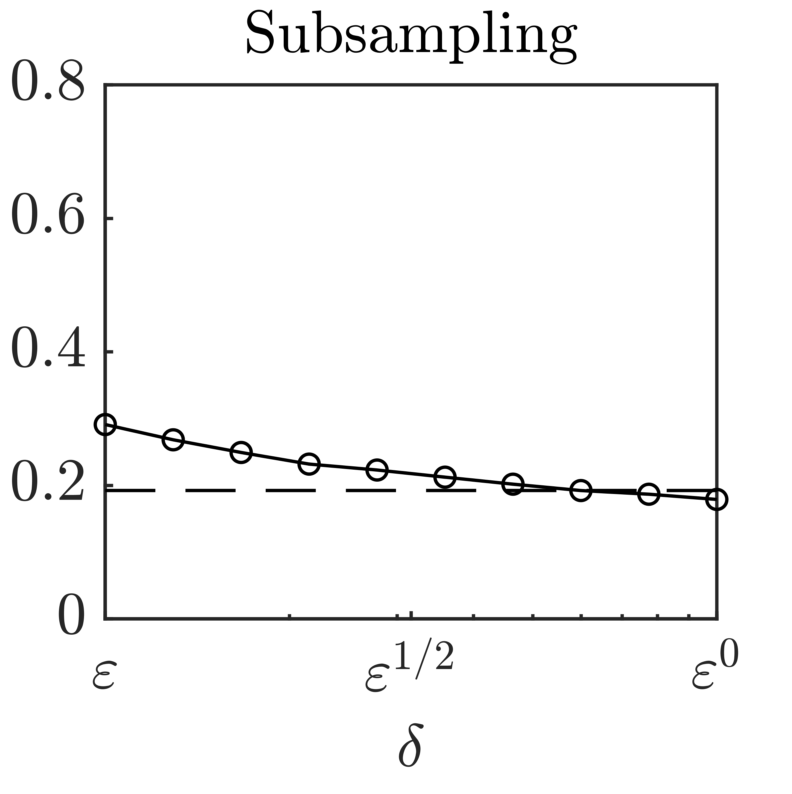
\includegraphics[]{Figures/OUSubs_s5} & 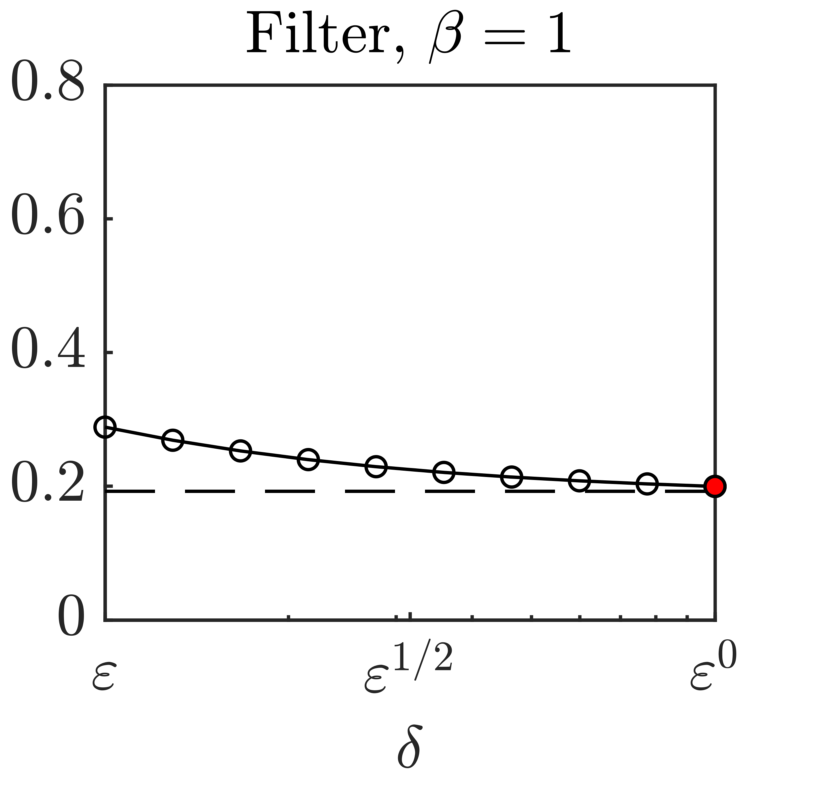
\includegraphics[]{Figures/OUFilt_s5_b1}  & 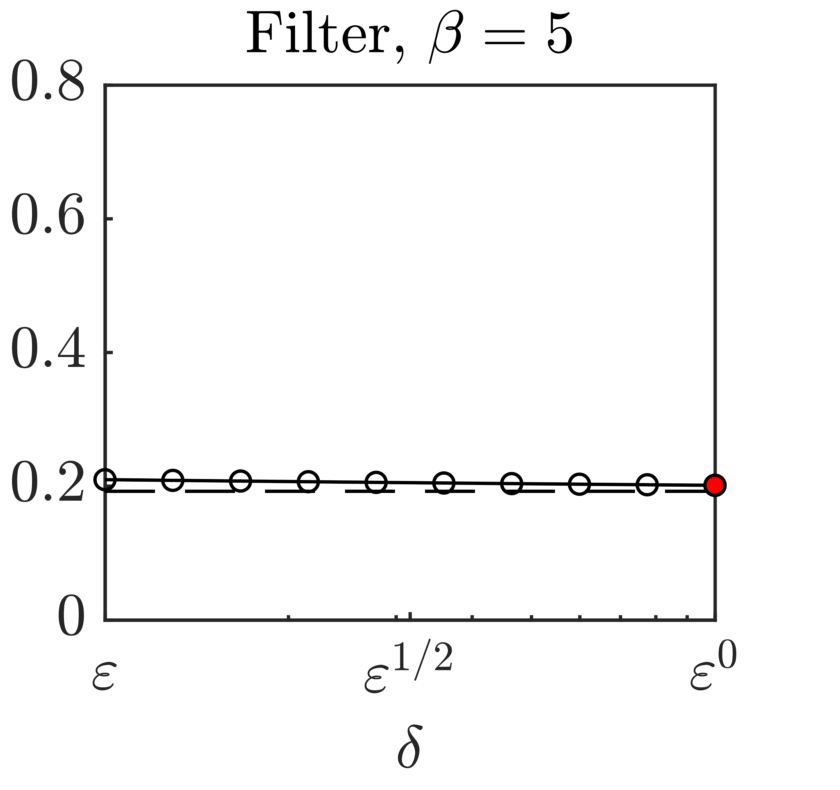
\includegraphics[]{Figures/OUFilt_s5_b5} \\ % & 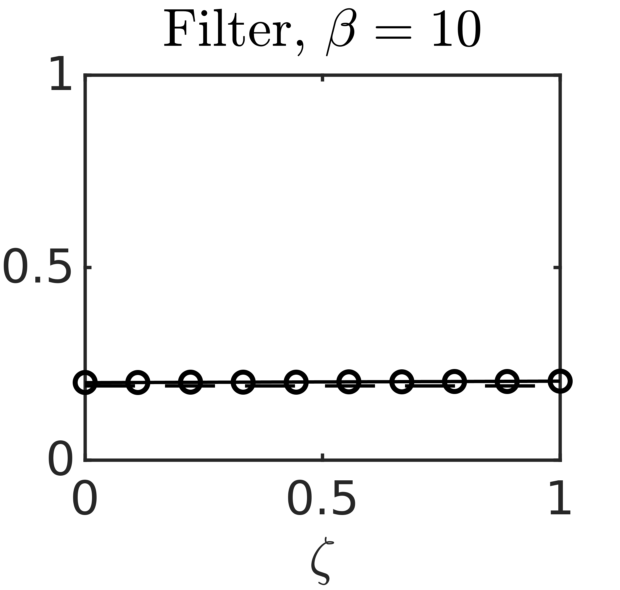
\includegraphics[]{Figures/OUFilt_s5_b10} \\
		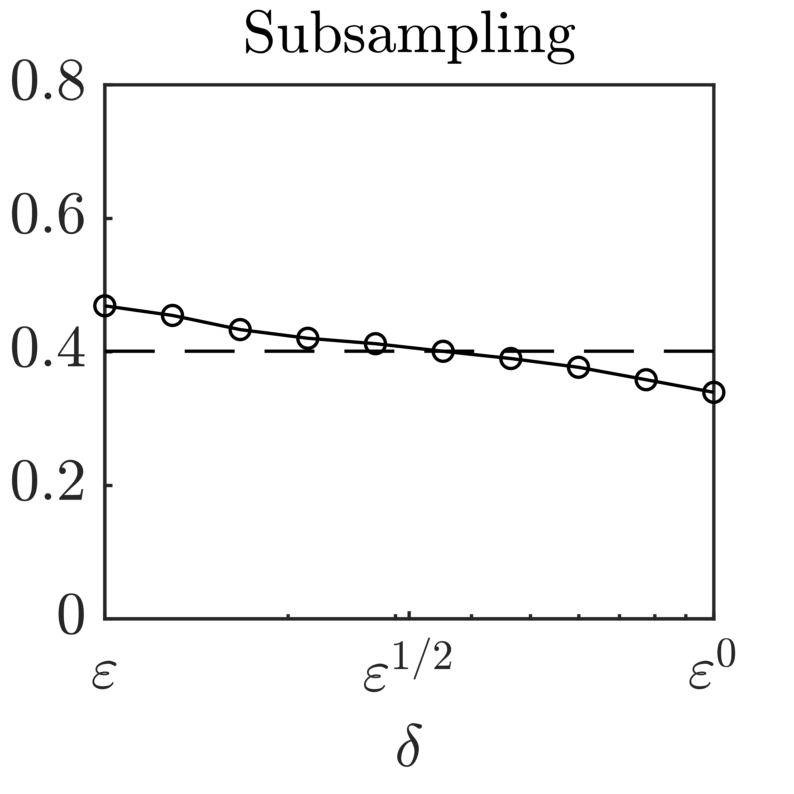
\includegraphics[]{Figures/OUSubs_s7} & 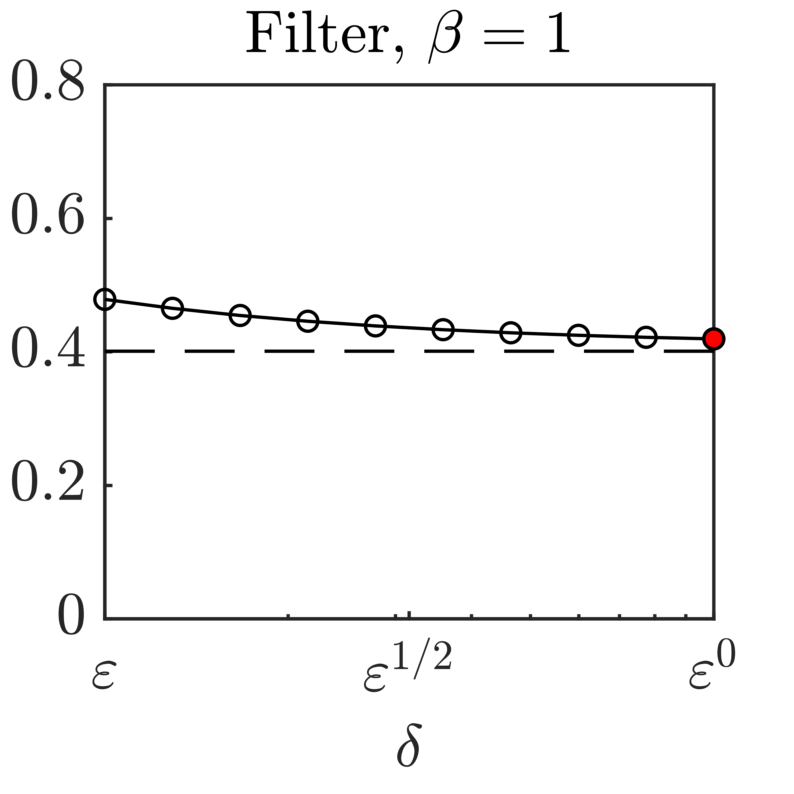
\includegraphics[]{Figures/OUFilt_s7_b1}  & 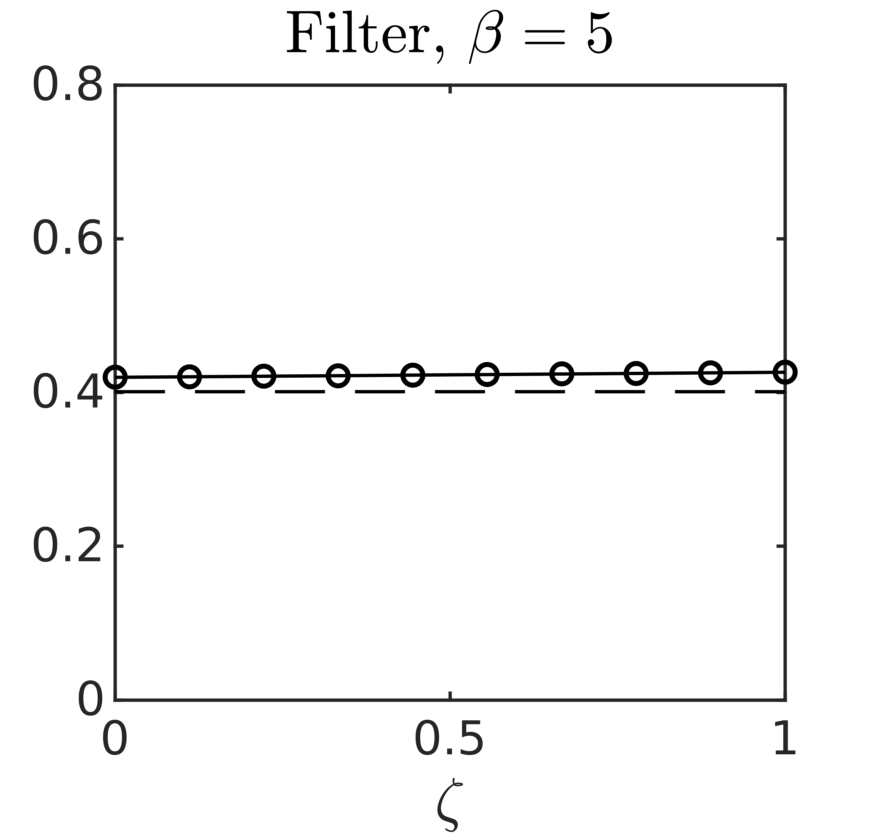
\includegraphics[]{Figures/OUFilt_s7_b5} \\ % & 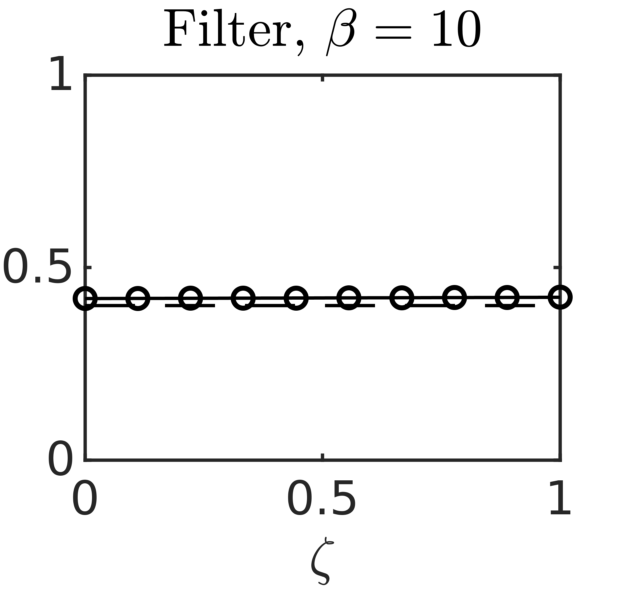
\includegraphics[]{Figures/OUFilt_s7_b10} \\
		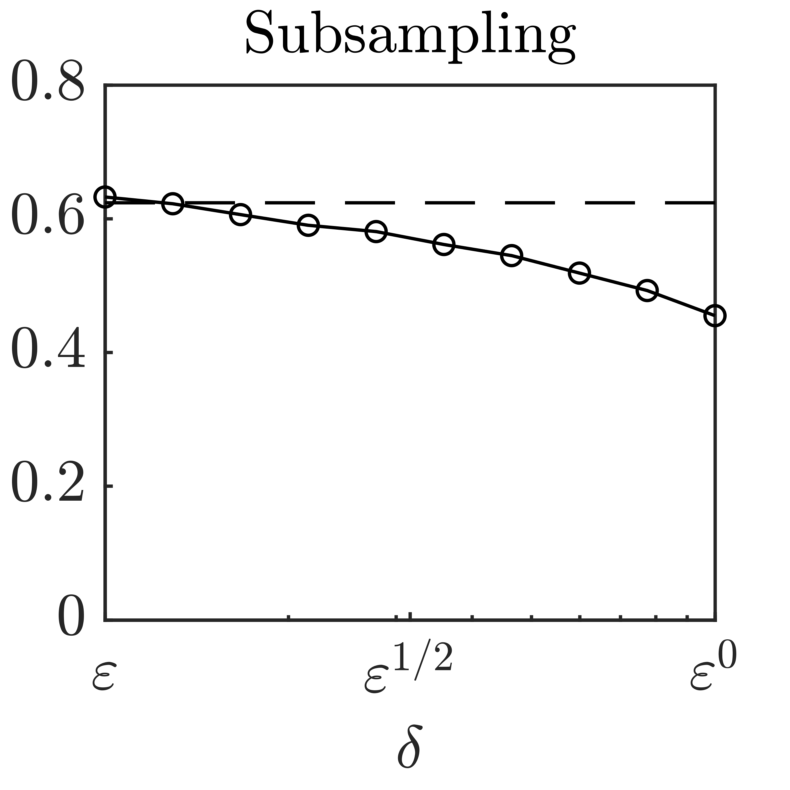
\includegraphics[]{Figures/OUSubs_s10} & 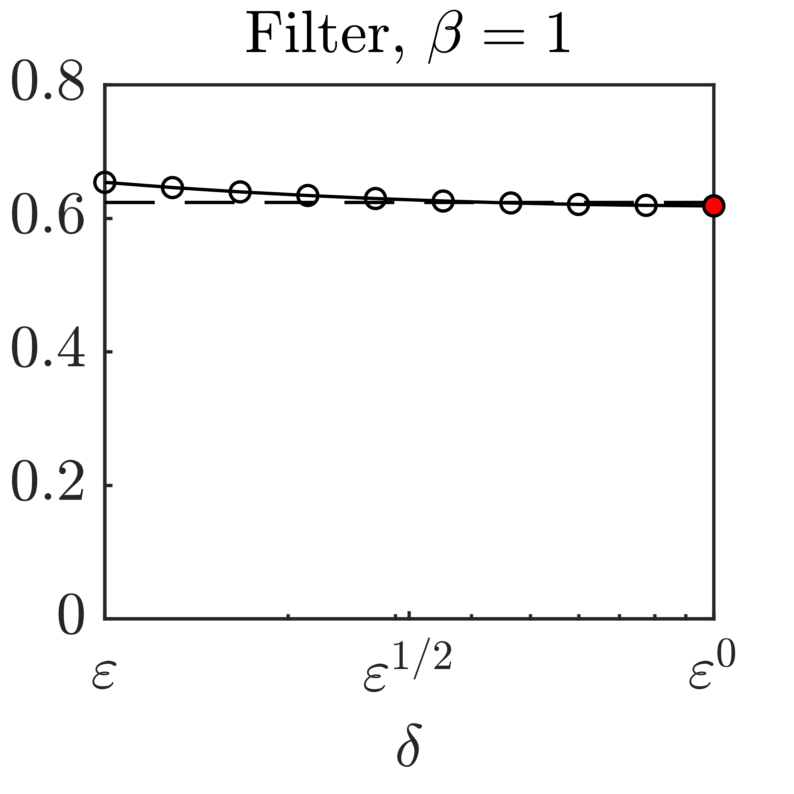
\includegraphics[]{Figures/OUFilt_s10_b1}  & 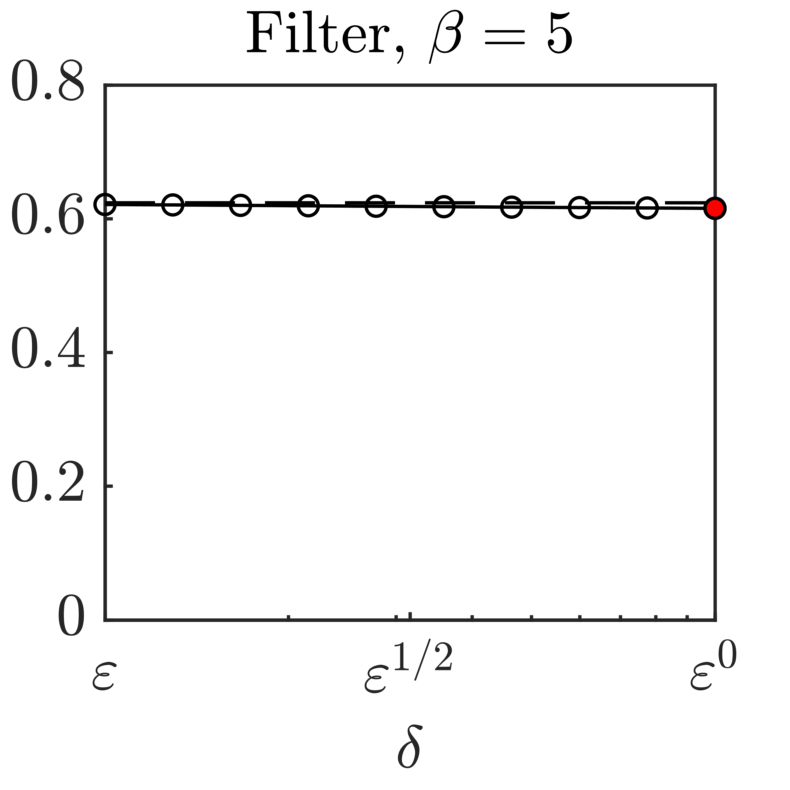
\includegraphics[]{Figures/OUFilt_s10_b5} % & 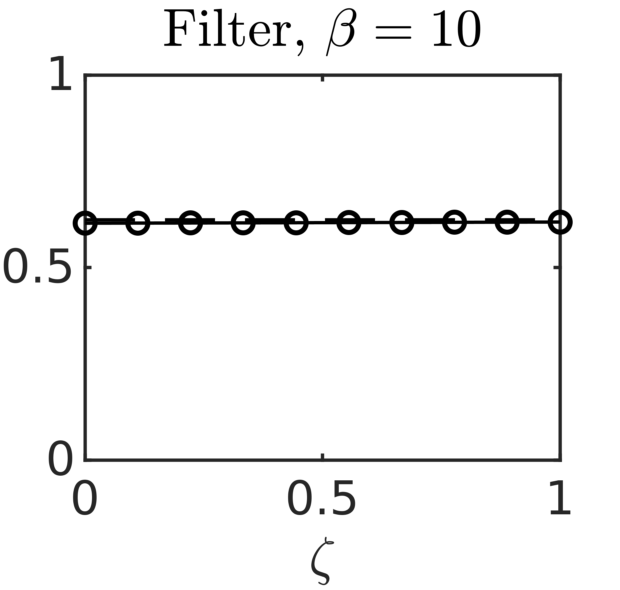
\includegraphics[]{Figures/OUFilt_s10_b10}
	\end{tabular}
	\caption{Results for the Ornstein--Uhlenbeck process. The axis of abscissae $\zeta$ represents the value of $\delta = \epl^\zeta$ for both subsampling and the filter. The three rows correspond to $\sigma = 0.5, 0.7, 1.0$ from top to bottom.}
	\label{fig:OU}
\end{figure}
We consider $N = 1$ and the quadratic potential $V(x) = x^2/2$. In this case, the solution of the homogenized equation is an Ornstein--Uhlenbeck process. Moreover, we set the multiscale equation \eqref{eq:SDE_MS} with $\epl = 0.1$ and the fast potential $p(y) = \cos(y)$. We generate data $X^\epl$ for $0 \leq t \leq T$ and $T = 10^3$ employing the Euler--Maruyama method with time step $\Delta_t = \epl^3$. 

As a first experiment, we consider the effect of setting different values of the parameter $\delta$ of the filter \eqref{eq:filter} on the estimator. As a comparison and for similarity with the subsampling approach, we consider $\delta = \epl^{\zeta}$ and vary $\zeta \in [0, 1]$. We employ the same values of $\delta$ for the subsampling, too, as the theoretical results guarantee convergence only for these values. Moreover, we repeat the experiments fixing $\beta = 1, 5$ and for three different values of the diffusion, i.e., we choose $\sigma = 0.5, 0.7, 1$. We report in Figure \ref{fig:OU} the experimental results. Let us remark that
\begin{enumerate}
	\item for $\sigma = 0.5$ the results given by subsampling and by the filter with $\beta = 1$ are similar, while for higher values of $\sigma$ the filtering approach seems better than subsampling, 
	\item in general, choosing a higher value of $\beta$ seems beneficial for the quality of the estimator,
	\item the dependence on $\delta$ of numerical results given by the filter seems relevant only in case $\beta = 1$ and for small values of $\sigma$. For $\beta = 1$ and higher values of $\sigma$, the estimator is stable with respect to this parameter, as predicted in Theorem \ref{thm:mainTheorem}. This can be observed for a higher value of $\beta$ but we have no theoretical guarantee in this case.
\end{enumerate}

As a second experiment, we therefore test the variability of the estimator with respect to $\beta$ in \eqref{eq:filter}. We repeat the numerical experiment in Figure \ref{fig:OU} and we choose to consider $\delta = \epl$, which corresponds to $\zeta = 1$ and seems to be the worst-case scenario for the filter, at least for $\beta = 1$. We consider again $\sigma = 0.5, 0.7, 1$ and vary $\beta = 1, 2, \ldots, 10$. Results, given in Figure \ref{fig:OUBeta}, show empirically that the estimator is fast stable with respect to $\beta$.

\begin{figure}[t]
	\centering
	\begin{tabular}{ccc}
		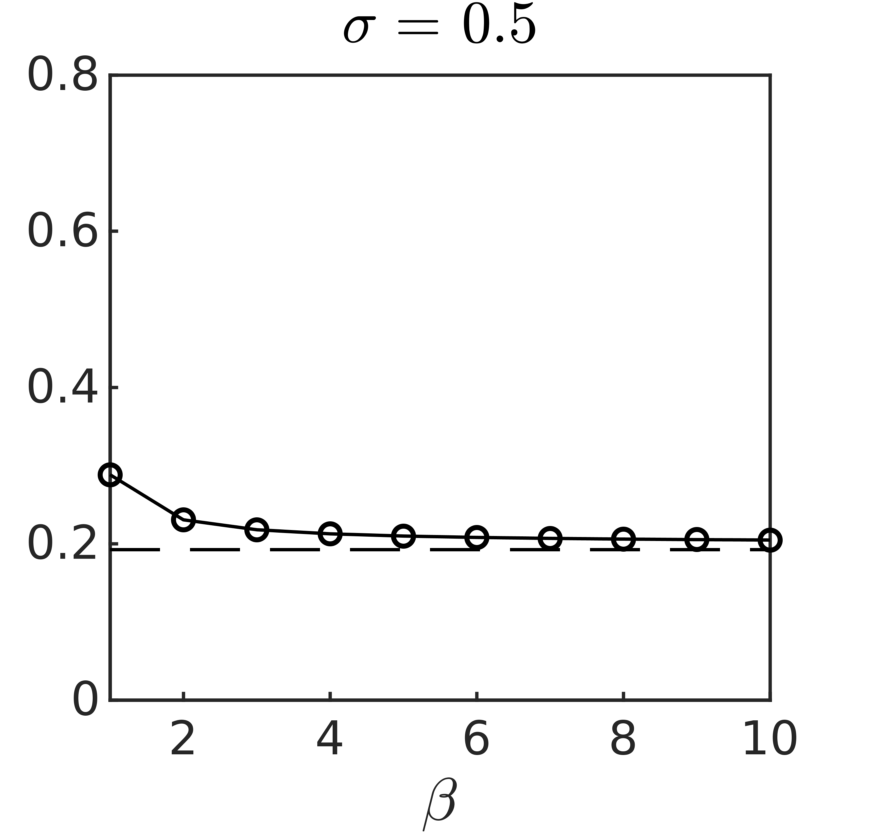
\includegraphics[]{Figures/OUBeta_s5} & 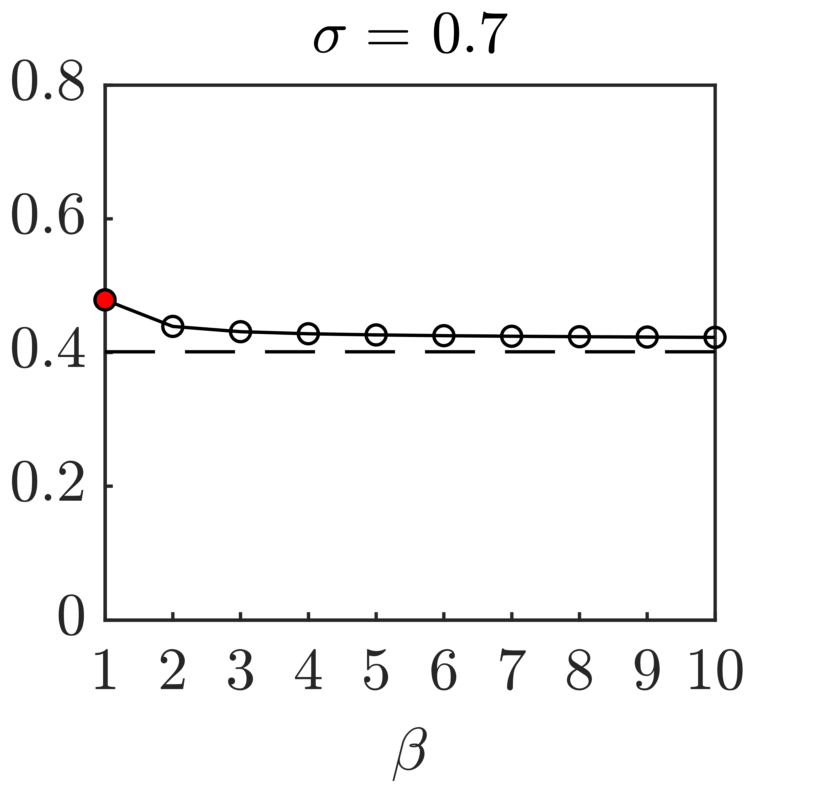
\includegraphics[]{Figures/OUBeta_s7}  & 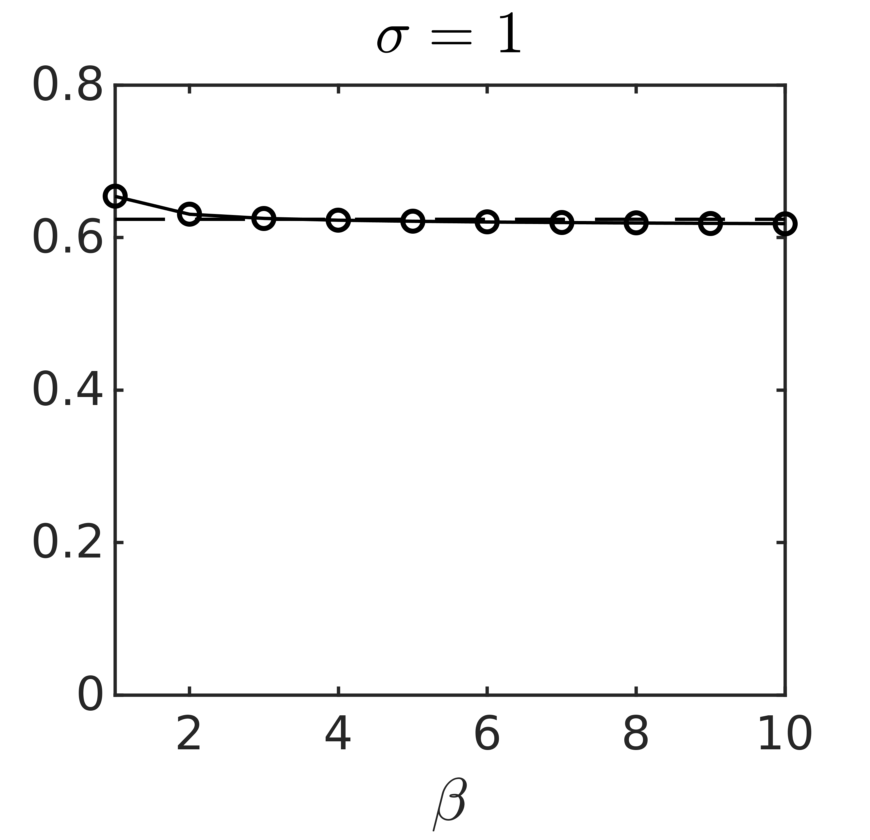
\includegraphics[]{Figures/OUBeta_s10} \\
	\end{tabular}
	\caption{Dependence of the estimator given by the filter for the Ornstein--Uhlenbeck process on the parameter $\beta$ in \eqref{eq:filter}. From left to right we consider different values of $\sigma$.}
	\label{fig:OUBeta}
\end{figure}

\subsection{The Bayesian approach: bistable potential}
\begin{figure}[t]
	\centering
	\begin{tabular}{ccc}
		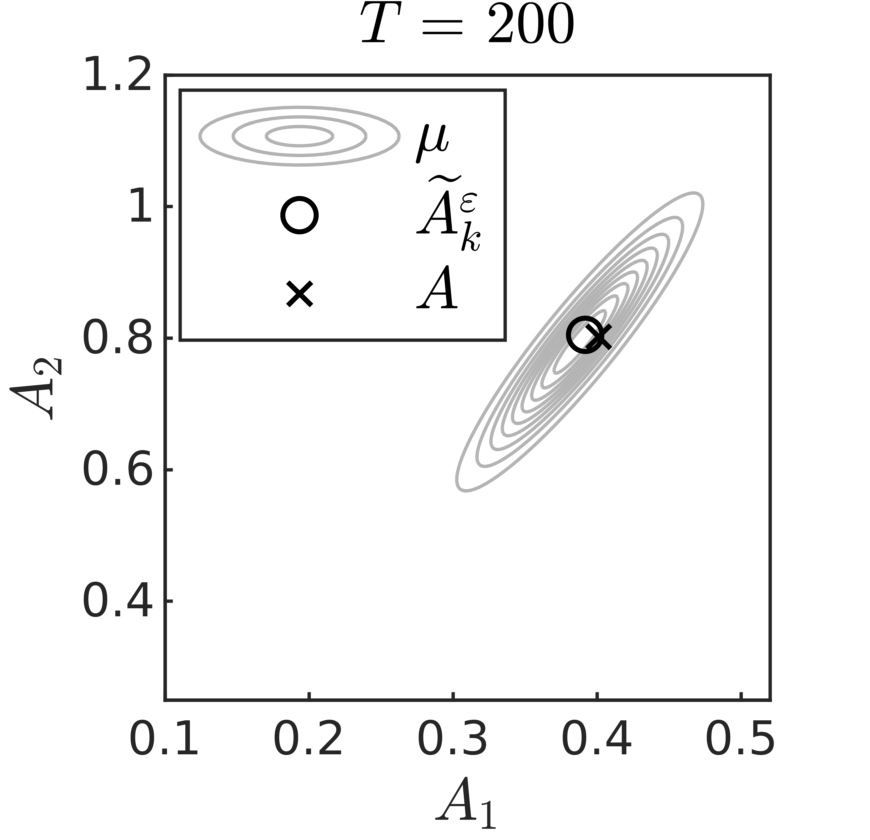
\includegraphics[]{Figures/Bayes_T200} & 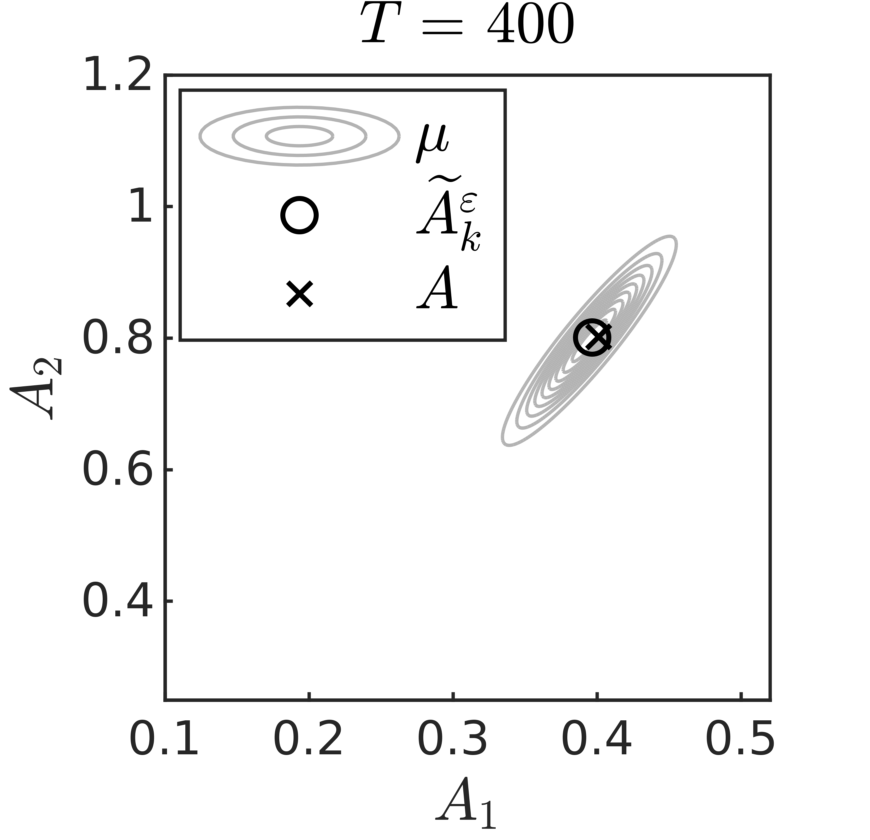
\includegraphics[]{Figures/Bayes_T400}  & 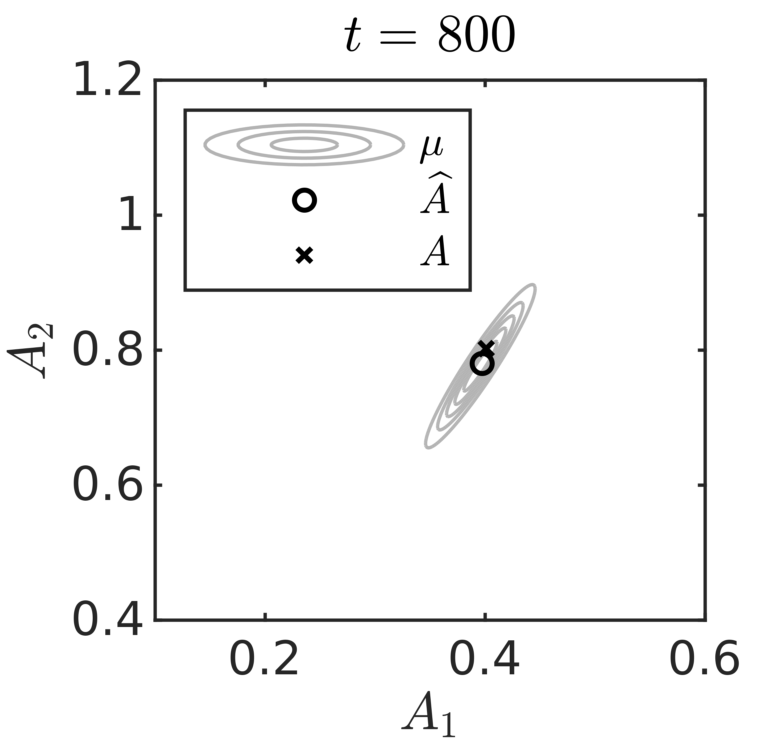
\includegraphics[]{Figures/Bayes_T800} \\
	\end{tabular}
	\caption{Posterior distributions over the parameter $A = (A_1, A_2)^\top$ for the bistable potential obtained with the filtering approach. The figures refer to time $t = 200, 400, 800$ from left to right, respectively. The MLE $\widehat A$ is represented with a circle, while the true value $A$ of the drift coefficient of the homogenized equation is represented with a cross.}
	\label{fig:Bayes}
\end{figure}

In this numerical experiment we consider $N = 2$ and the bistable potential, i.e., the function $V$ defined as
\begin{equation}
	V(x) = \begin{pmatrix} \dfrac{x^4}{4} & \dfrac{x^2}{2} \end{pmatrix}^\top,
\end{equation}
with coefficients $\alpha_1 = 1$ and $\alpha_2 = -2$. We then consider the multiscale equation with $\sigma = 0.8$, the fast potential $p(y) = \cos(y)$ and $\epl = 0.05$, thus simulating a trajectory $X^\epl$ for time $0 \leq t \leq T$, with $T = 800$. We adopt here a Bayesian approach and compute the posterior distribution $\mu(A \mid X^\epl)$ obtained with the filtering approach. The filter's parameters are set to $\beta = 1$ and $\delta = \epl^{1/2}$ in \eqref{eq:filter}. Let us remark that in order to compute the posterior covariance the diffusion coefficient $\Sigma$ of the homogenized equation has to be known. In this case, we pre-compute the value of $\Sigma$ via the coefficient $K$ and the theory of homogenization, but let us remark that $\Sigma$ could be estimated employing the subsampling technique of \cite{PaS07}. We stop computations at times $t = 200, 400, 800$ in order to observe the shrinkage of the Gaussian posterior towards the MLE with respect to time. In Figure \ref{fig:Bayes}, we observe that the posterior does indeed shrink towards the MLE, which in turn gets progressively closer to the true value of the drift coefficient $A$ of the homogenized equation.


\subsection{Multi-dimensional parameter}

\begin{figure}[t]
	\centering
	\begin{tabular}{ccc}
		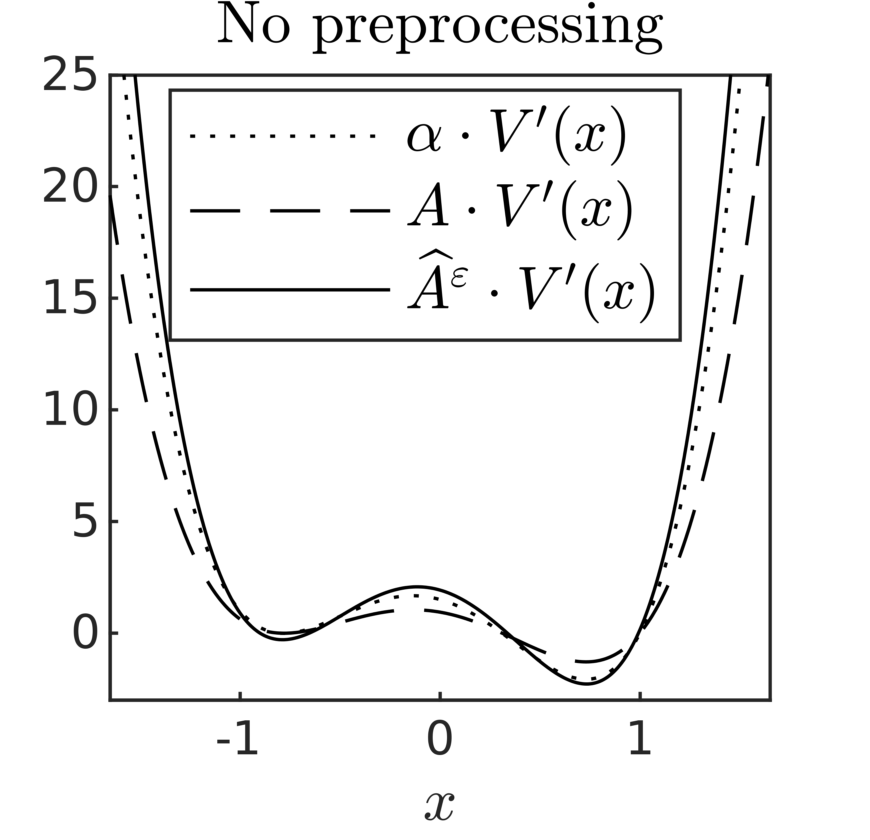
\includegraphics[]{Figures/KLNothing} & 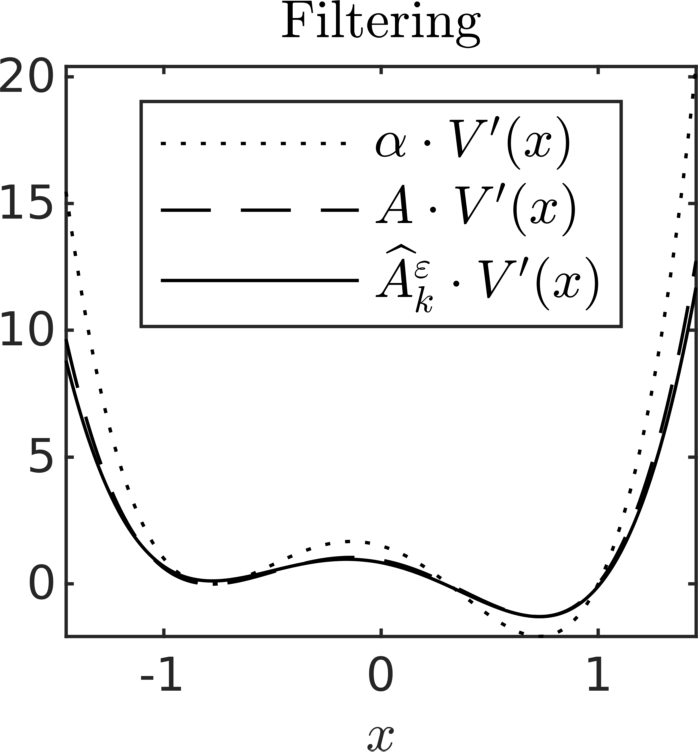
\includegraphics[]{Figures/KLFilt}  & 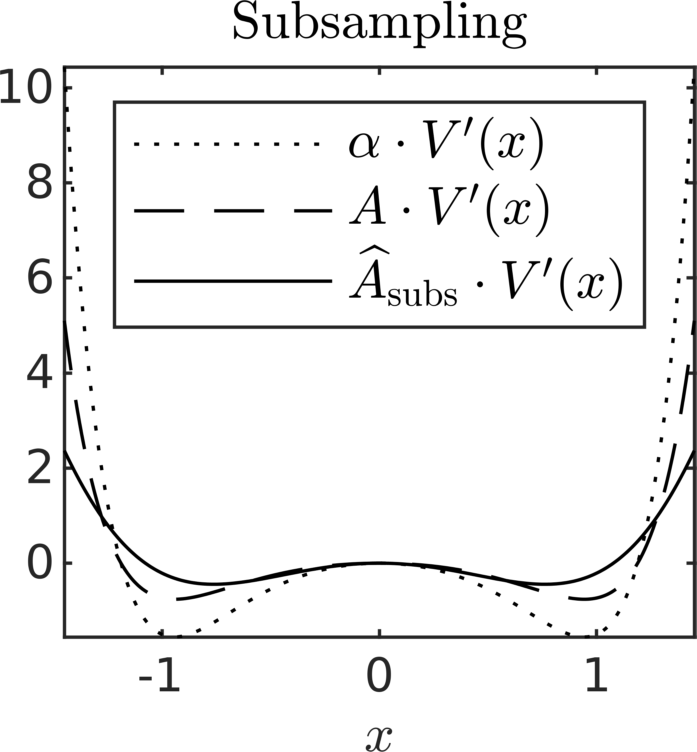
\includegraphics[]{Figures/KLSubs}
	\end{tabular}
	\caption{Results for the four-dimensional parameters. From left to right the potential function estimated with (i) the data itself, (ii) the filter, (iii) subsampled data.}
	\label{fig:KLStyle}
\end{figure}

We consider $N = 4$ and the potential function $V(x)$ as in \eqref{eq:Potential} with
\begin{equation}
	V_i(x) = \frac{x^{2i}}{2i}, \quad i =1, \ldots, 4,
\end{equation}
so that $\alpha \cdot V'(x) = \alpha_1 x + \alpha_2 x^3 + \alpha_3 x^5 + \alpha_4 x^7$, with $\alpha = (-2, -1, 1, 1/2)$. We consider $\epl = 0.05$, the fast potential $p(y) = \cos(y)$ and simulate a trajectory of $X^\epl$ for $0 \leq t \leq T$ with $T = 10^3$ employing the Euler--Maruyama method with time step $\Delta_t = \epl^3$. We compute the MLE of the drift coefficient $A \in \R^4$ of the homogenized equation \eqref{eq:SDE_HOM} employing 
\begin{enumerate}
	\item the data $X^\epl$ itself,
	\item subsampled data with subsampling parameter $\delta = \epl^{2/3}$,
	\item filtered data $Z^\epl$ computed with $\beta = 1$ and $\delta = 0.2$.
\end{enumerate}
In particular, we pick this specific value of $\delta$ for the subsampling following the optimality criterion given in \cite{PaS07}. Results, given in Figure \ref{fig:KLStyle}, show that the filter-based estimation captures well the homogenized potential.


\bibliographystyle{siam}
\bibliography{anmc}
\end{document}  
